\section{Knoten und Äquivalenzklassen}

\subsection{Repräsentation von Relationen}
\label{sec:Bitvector}

Die einzelnen Relationen werden mit Hilfe eines Bitvektors dargestellt. Jeder Basis-Relation - sie repräsentiert eine physische Relation - ist eine ID zugeordnet. Eine Basis-Relation wird in diesem Prototypen mit Hilfe eines auf \texttt{TRUE} gesetzten Bits in einem Bitvektor repräsentiert. Auch mehrere Relationen können durch einen Bitvektor abgebildet werden dazu werden mehrere Bits auf \texttt{TRUE} gesetzt.

\subsubsection{Implementierung}

Als Basis für die Implementierung dient ein Bitvektor. Ein Bitvektor sind mehrere Bits, die entweder \texttt{TRUE} also \texttt{1} oder \texttt{FALSE} also \texttt{0} sein können. Ist das n-te Bit eines Bitvektors gesetzt, so repräsentiert dieses Bit die n-te Relation. Beispielsweise bezeichnet der Bitvektor \texttt{010000000} die Relation mit der ID \texttt{1}. Mit Hilfe des Bitvektors können auch mehrere Relationen gespeichert werden \texttt{01010000000} bezeichnet folglich die Relation mit dem Name \texttt{1} und die Relation mit der ID \texttt{3}. Für die durchgeführten Berechnungen ist es nicht notwendig, dass eine Relation mit ihrem tatsächlichen Namen bekannt ist. Es reicht eine Bezeichnung mit Hilfe von Nummern aus.

Vorteil für die Verwendung von Bitvektoren ist, dass einfach Mengenoperationen durchgeführt werden können. So kann einfach geprüft werden, ob Äquivalenzklassen gemeinsame JOIN Kanten besitzen oder neue Relationen einer Äquivalenzklasse hinzugefügt werden. (vgl. Abb. \ref{Bitvector}) Dies ist besonders effizient, da nur Bits und keine komplexen Objekte wie Strings verarbeitet werden müssen.



\begin{figure}[ht]
  \centering
  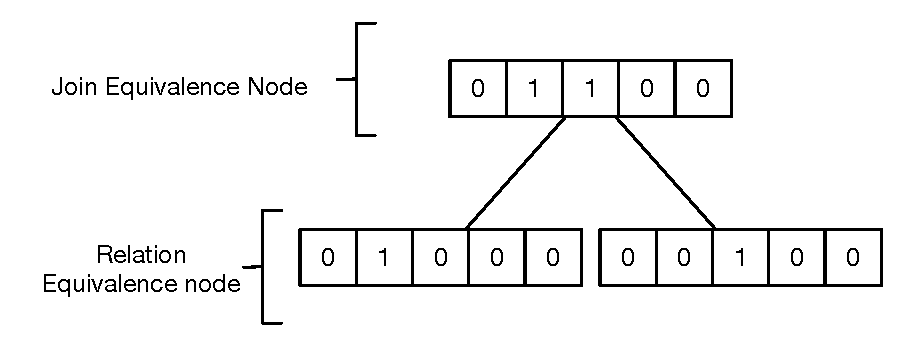
\includegraphics{04_Implementierung/Bitvector.pdf}
  \caption{Bitvekotren als Repräsentation von Relationen oder Joins}
  \label{Bitvektor}
\end{figure}


Die konkrete Erzeugung von Bitvektoren zu repräsentation von Relationen entsteht bei der Erstellung neuer Pläne bzgl. Äquivalenzklassen. Bezeichnet eine Äquivalenzklasse nur eine Basis-Relation so ist ihr Bitevektor \texttt{\_relations} auf nur einen Wert gesetzt. Wird einer Äuqivalenzklasse ein Planknoten hinzugefügt, wird die Variable \texttt{\_relations} mit den Relationen, die links bzw. rechts an einem Plan-Knoten hängen angereichert.



\subsubsection{Erweiterbarkeit}
Die Implementierung des Bitvektors erlaubt es mit Hilfe eines Templateparameters die Länge des Bitevektors anzupassen.



\subsection{Planknoten und Äquivalenzklassen}




\begin{figure}[ht]
  \centering
  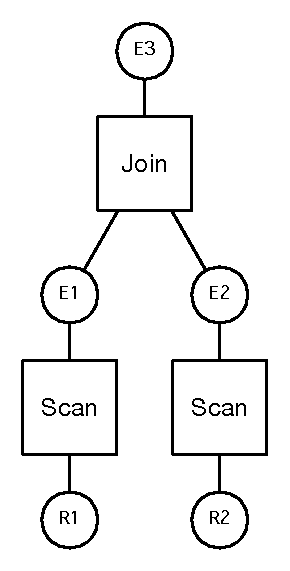
\includegraphics{04_Implementierung/JoinScan.pdf}
  \caption{Planknoten und Äquivalenzklassen}
  \label{PlanAequi}
\end{figure}

Die Datenstruktur in der Pläne gespeichert sind sind sowohl \texttt{Plannode} und \texttt{EquivalenceClasses}. Einem Planknoten ist ein Operator zugewiesen. Beispielsweise \texttt{JOIN} oder \texttt{SCAN}. In \texttt{EquivalenceClass} werden mehrere Pläne gespeichert, die alle semantisch gleich sind. Ein einfaches Beispiel ist in Abbildung \ref{PlanAequi} zu finden. Ein einfacher Plan bestehend aus einem Join und zwei Scans ist zu sehen. Der oberste Knoten \texttt{E3} ist eine Äquivalenzklasse in Ihr findet sich der erste Planknoten ein Join. Der Join hat zwei Seiten eine linke und eine rechte. Beide Seiten sind mit einer Äquivalenzklasse verbunden \texttt{E1} resp. \texttt{E2}. Die jeweils einen Scan beinhalten, der die Basis-Relationen \texttt{R1} bzw. \texttt{R2} einliesst. Die Beiden Basis-Relationen sind ebenso wie die Äquivalenzklassen als \texttt{EquivalenceClass} im System abgelegt.




\subsubsection{Implementierung}

\begin{figure}[ht]
  \centering
  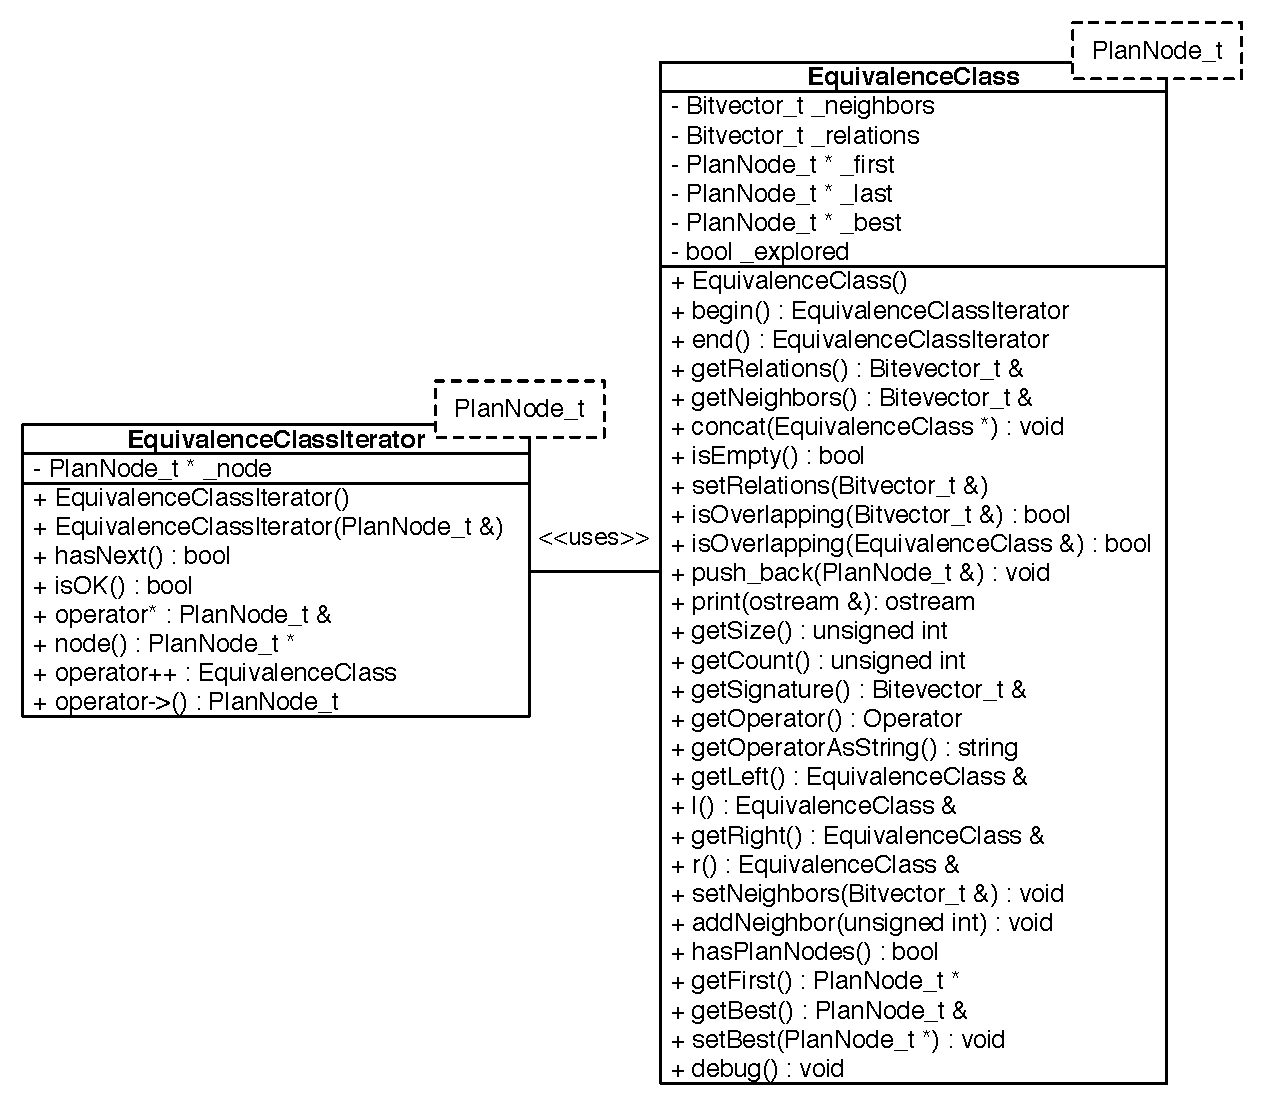
\includegraphics[width=1\textwidth]{04_Implementierung/ClassEquivalenceClass.pdf}
  \caption{Klassendiagramm: Äquivalenzklasse}
  \label{ClassEquivalenceClass}
\end{figure}

\subsubsection{Erweiterbarkeit}

